\question[6] 1.下列说法正确的是
\begin{center}
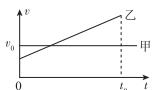
\includegraphics[]{img/image1.jpeg}
\end{center}

\fourchoices{加速度为正值,物体一定做加速直线运动}{百米比赛时,运动员的冲刺速度越大成绩越好}{做直线运动的物体,加速度为零时,速度不一定为零,速度为零时,加速度一定为零}{相对于某参考系静止的物体,对地速度不一定为零}
\begin{solution}{4cm}

\end{solution}



\question[6] 密目2.小球在水中运动时受到水的阻力与小球运动速度的平方成正比,即f=kv,则比例系数k的单位是
\fourchoices{$kg·m^2$}{kg·m}{$kg/m^2$}{$kg/m^2$}
\begin{solution}{4cm}

\end{solution}



\question[6] ⋮目3.正在海上行驶的一艘帆船,行驶方向如图所示,海风吹来的方向与船行驶的方向夹角为53°,升起风帆,调整风帆的角度,使海风垂直吹在帆面上,若海风吹在帆面上的风力大小为500N,则沿船行驶方向获得的推力大小为(sin53°=0.8,cos53∘=0.6)
\begin{center}
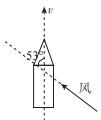
\includegraphics[]{img/image3.jpeg}
\end{center}

\fourchoices{300N}{375N风}{目400N450N}{400N450N}
\begin{solution}{4cm}

\end{solution}



\question[6] 4.可看作质点的甲、乙两汽车沿着两条平行车道直线行驶,在甲车匀速路过A处的同时,乙车从此处由静止匀加速启动,从某时刻开始计时,两车运动的v━t图象黑目如图所示,$t_b$时刻在B处甲、乙两车相遇.下面说法正确的是一甲
\begin{center}
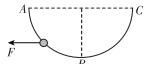
\includegraphics[]{img/image4.jpeg}
\end{center}

\fourchoices{A,B两处的距离为$v_0$$t_0$}{t.时刻乙车的速度是2$v_0$}{t=0时刻两车并排行驶}{t=0时刻乙车行驶在甲车前面}
\begin{solution}{4cm}

\end{solution}



\question[6] 5.如图所示,木箱置于水平地面上,一轻质弹簧一端固定在木箱顶部,另一端系一小球,小球下端用细线拉紧固定在木箱底部.剪断细线,小球上下运动过程中木箱刚好不能离开地面.已知小球和木箱的质量相同,重力加速度大小为g,若$t_0$时刻木箱刚好不能离开地面,下面说法正确的是

\begin{solution}{4cm}

\end{solution}



\question[6] 6.如图所示,A,B两个小球用长为1m的细线连接,用手拿着A球,B球竖直悬挂,且A、B两球均静止.现由静止释放A球,测得两球落地的时间差为0.2s,不计空气阻力,重力加速度g=$10m/s^2$,则A球释放时离地面的高度为
\begin{center}
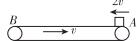
\includegraphics[]{img/image6.jpeg}
\end{center}

\fourchoices{1.25m}{1.80mB●}{3.60m6.25m}{3.60m6.25m}
\begin{solution}{4cm}

\end{solution}



\question[6] 7.如图所示,A、B,C,D四个小球质量分别为m、4m,2m、3m,用细线连着,在A和C之间细线上还串接有一段轻弹簧,悬挂在光滑定滑轮的两边并处于静止状态.弹簧的形变在弹性限度内,叫重力加速度大小为g,则下列说法正确的是
\begin{center}
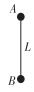
\includegraphics[]{img/image7.jpeg}
\end{center}

\fourchoices{剪断C,D间细线的一瞬间,小球C的加速度大小为3g}{剪断C,D间细线的一瞬间,小球A和B的加速度大小均为$\frac{3}{7}$g}{剪断A、B间细线的一瞬间,小球C的加速度大小为零B●}{剪断C球上方细线的一瞬间,小球A和B的加速度大小均为零}
\begin{solution}{4cm}

\end{solution}



\question[6] 8.某人提着箱子站在电梯里,电梯从一楼上升到三楼的整个过程中先匀加速后匀减速,关于此过程,下列说法正确的是
\fourchoices{手对箱子的力大小始终等于箱子对手的力的大小}{手对箱子的力大小始终等于箱子的重力的大小}{人对电梯的压力先持续增大后持续减小}{人对电梯的压力先大于人和箱子的总重力后小于人和箱子的总重力}
\begin{solution}{4cm}

\end{solution}



\question[6] 9.将一个小球竖直向上抛出,碰到高处的天花板后反弹,并竖直向下运动回到抛出点,若反弹的速度大小是碰撞前速度大小的0.65倍,小球上升的时间为1s,下落的时间为1.2s,重力加速度取$10m/s^2$,不计空气阻力和小球与天花板的碰撞时间,则下列说法正确的是
\begin{center}
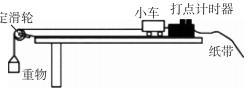
\includegraphics[]{img/image9.jpeg}
\end{center}

\fourchoices{小球与天花板碰撞前的速度大小为10m/s}{小球与天花板碰撞前的速度大小为8m/s}{抛出点到天花板的高度为15m}{抛出点到天花板的高度为13m}
\begin{solution}{4cm}

\end{solution}



\question[6] 10.如图所示,半圆ABC是由一条光滑的杆弯曲而成的.带有小孔的小球穿在杆上,在水平拉力F的作用下小球由B点开始缓慢升高,此过程中半圆ABC竖直固定不动,AC连线水平.在小球缓慢上升的过程中,有关水平拉力F、杆对小球的作用力$F_N$的变化情况,下列说法正确的是
\fourchoices{F逐渐变大}{F逐渐变小}{$F_N$逐渐变大$F_N$逐渐变小}{$F_N$逐渐变大$F_N$逐渐变小}
\begin{solution}{4cm}

\end{solution}



\question[6] 11.如图所示,水平传送带以大小为v的速率沿顺时针匀速运行,一个小物块从传送带的右端点A以大小为2v的速度向左滑上传送带,小物块滑到传送带正中间时速度减为零.已知小物块与传送带间的动摩擦因数为μ,重力加速度为g,则下列说法正确的是
\begin{center}
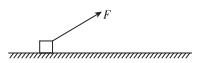
\includegraphics[]{img/image11.jpeg}
\end{center}

\fourchoices{A,B两点间的距离为$\frac{2v^{2}}{ \mu g}$}{小物块在传送带上运动时与传送带的相对位移为$\frac{9v^{2}}{2 \mu g}$}{要使小物块从传送带左端点B滑离,小物块在右端点A滑上传送带的速度至少为3v}{增大传送带的速度(仍小于2v),小物块与传送带间相对运动的时间变长}
\begin{solution}{4cm}

\end{solution}



\question[6] 12.质量为m的物块放在水平桌面上,物块与水平桌面间的动摩擦因数为$\frac{\sqrt{3}}{3}$现给物块一个斜向上的拉力F使物块匀速向右运动,则拉力F的值可能为
\begin{center}
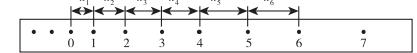
\includegraphics[]{img/image12.jpeg}
\end{center}

\fourchoices{$\frac{1}{4}$mg}{$\frac{1}{3}$mg}{$\frac{1}{2}$mgmg}{$\frac{1}{2}$mgmg}
\begin{solution}{4cm}

\end{solution}



